


\begin{applicationActivities}



\begin{definition}
  A \term{basis} is a linearly independent set that spans a vector space.

  \vspace{1em}

  The \term{standard basis} of \(\IR^n\) is the set \(\{\vec{e}_1, \ldots, \vec{e}_n\}\) where
  \begin{align*}
  \vec{e}_1 &= \begin{bmatrix}1 \\ 0 \\ 0 \\ \vdots \\ 0 \\  0 \end{bmatrix} &
  \vec{e}_2 &= \begin{bmatrix}0 \\ 1 \\ 0 \\ \vdots \\ 0 \\ 0 \end{bmatrix} &
  \cdots & &
  \vec{e}_n = \begin{bmatrix}0 \\ 0 \\ 0 \\ \vdots \\ 0 \\ 1 \end{bmatrix}
  \end{align*}

  \vspace{1em}

  For \(\IR^3\), these are the vectors
  \(
    \vec e_1=\hat\imath=\begin{bmatrix}1 \\ 0 \\ 0\end{bmatrix},
    \vec e_2=\hat\jmath=\begin{bmatrix}0 \\ 1 \\ 0\end{bmatrix},
  \) and \(
    \vec e_3=\hat k=\begin{bmatrix}0 \\ 0 \\ 1\end{bmatrix}
  \).

  \end{definition}

\begin{observation}
  A basis may be thought of as a collection of building blocks for a vector
  space,  since every vector in the space can be expressed as a unique linear
  combination of basis vectors.

  \vspace{1em}

  For example, in many calculus courses, vectors in \(\IR^3\)
  are often expressed in their component form
  \[
    (3,-2,4)=\begin{bmatrix}3 \\ -2 \\ 4\end{bmatrix}
  \]
  or in their standard basic vector form
  \[
    3\vec e_1-2\vec e_2+4\vec e_3 = 3\hat\imath-2\hat\jmath+4\hat k
  .\]
  Since every vector in \(\IR^3\) can be uniquely described as a linear
  combination of the vectors in \(\setList{\vec e_1,\vec e_2,\vec e_3}\),
  this set is indeed a basis.
\end{observation}



\begin{activity}{15}
  Label each of the sets \(A,B,C,D,E\) as
  \begin{itemize}
     \item SPANS \(\IR^4\) or DOES NOT SPAN \(\IR^4\)
     \item LINEARLY INDEPENDENT or LINEARLY DEPENDENT
     \item BASIS FOR \(\IR^4\) or NOT A BASIS FOR \(\IR^4\)
  \end{itemize}
  by finding \(\RREF\) for their corresponding matrices.
  \begin{center}
    \begin{tabular}{cc}
  	\(A=\left\{
      \begin{bmatrix}1\\0\\0\\0\end{bmatrix},
      \begin{bmatrix}0\\1\\0\\0\end{bmatrix},
      \begin{bmatrix}0\\0\\1\\0\end{bmatrix},
      \begin{bmatrix}0\\0\\0\\1\end{bmatrix}
      \right\}
      \)   &

    \(B=\left\{
      \begin{bmatrix}2\\3\\0\\-1\end{bmatrix},
      \begin{bmatrix}2\\0\\0\\3\end{bmatrix},
      \begin{bmatrix}4\\3\\0\\2\end{bmatrix},
      \begin{bmatrix}-3\\0\\1\\3\end{bmatrix}
      \right\}
      \)  \\


      \(C=\left\{
      \begin{bmatrix}2\\3\\0\\-1\end{bmatrix},
      \begin{bmatrix}2\\0\\0\\3\end{bmatrix},
      \begin{bmatrix}3\\13\\7\\16\end{bmatrix},
      \begin{bmatrix}-1\\10\\7\\14\end{bmatrix},
      \begin{bmatrix}4\\3\\0\\2\end{bmatrix}
      \right\}
      \) &

  	\(D=\left\{
      \begin{bmatrix}2\\3\\0\\-1\end{bmatrix},
      \begin{bmatrix}4\\3\\0\\2\end{bmatrix},
      \begin{bmatrix}-3\\0\\1\\3\end{bmatrix},
      \begin{bmatrix}3\\6\\1\\5\end{bmatrix}
      \right\}
      \) \\

     \(E=\left\{
      \begin{bmatrix}5\\3\\0\\-1\end{bmatrix},
      \begin{bmatrix}-2\\1\\0\\3\end{bmatrix},
      \begin{bmatrix}4\\5\\1\\3\end{bmatrix}
      \right\}
      \)  &
    \end{tabular}
  \end{center}
\end{activity}

\begin{activity}{10}
  If \(\{\vect v_1,\vect v_2,\vect v_3,\vect v_4\}\) is a basis for
  \(\IR^4\), that means \(\RREF[\vect v_1\,\vect v_2\,\vect v_3\,\vect v_4]\)
  doesn't have a non-pivot column, and doesn't have a
  row of zeros. What is \(\RREF[\vect v_1\,\vect v_2\,\vect v_3\,\vect v_4]\)?

  \[
    \RREF[\vect v_1\,\vect v_2\,\vect v_3\,\vect v_4]
      =
    \begin{bmatrix}
      \unknown & \unknown & \unknown & \unknown \\
      \unknown & \unknown & \unknown & \unknown \\
      \unknown & \unknown & \unknown & \unknown \\
      \unknown & \unknown & \unknown & \unknown \\
    \end{bmatrix}
  \]
\end{activity}

\begin{fact}
  The set \(\{\vect v_1,\dots,\vect v_m\}\) is a basis for \(\IR^n\) if and
  only if \(m=n\) and
  \(\RREF[\vect v_1\,\dots\,\vect v_n]=
  \begin{bmatrix}
    1&0&\dots&0\\
    0&1&\dots&0\\
    \vdots&\vdots&\ddots&\vdots\\
    0&0&\dots&1
  \end{bmatrix}
  \).

  That is, a basis for \(\IR^n\) must have exactly \(n\) vectors and
  its square matrix must row-reduce to the so-called \term{identity matrix}
  containing all zeros except for a downward diagonal of ones.
  (We will learn where the identity matrix gets its name in a later module.)
\end{fact}

\begin{observation}
Recall that a \textbf{subspace} of a vector space is a subset that is itself a vector space.

\vspace{1em}

One easy way to construct a subspace is to take the span of set,
but a linearly dependent set contains ``redundant'' vectors. For example,
only two of the three vectors in the following image are needed to span
the planar subspace.

\begin{center}
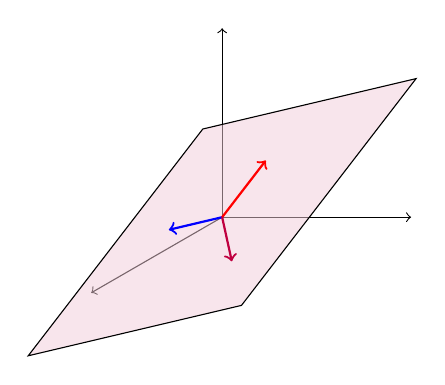
\begin{tikzpicture}[x={(210:0.8cm)}, y={(0:1cm)}, z={(90:1cm)},scale=0.4]
  \draw[->] (0,0,0) -- (6,0,0);
  \draw[->] (0,0,0) -- (0,6,0);
  \draw[->] (0,0,0) -- (0,0,6);
  \draw[fill=purple!20,fill opacity=0.5]
    (-2,-2,2) -- (6,-2,-2) -- (2,2,-2) -- (-6,2,2) -- (-2,-2,2);
  \draw[thick,blue,->] (0,0,0) -- (1,-1,0);
  \draw[thick,red,->] (0,0,0) -- (-2,0,1);
  \draw[thick,purple,->] (0,0,0) -- (1,1,-1);
\end{tikzpicture}
\end{center}
\end{observation}

\begin{activity}{10}
  Consider the subspace \(W=\vspan\left\{
  \begin{bmatrix}2\\3\\0\\1\end{bmatrix},
  \begin{bmatrix}2\\0\\1\\-1\end{bmatrix},
  \begin{bmatrix}2\\-3\\2\\-3\end{bmatrix},
  \begin{bmatrix}1\\5\\-1\\0\end{bmatrix}
  \right\}
  \) of \(\IR^4\).

  \begin{subactivity}
    Mark the part of \(\RREF\begin{bmatrix}
    2&2&2&1\\
    3&0&-3&5\\
    0&1&2&-1\\
    1&-1&-3&0
    \end{bmatrix}\) that shows that \(W\)'s spanning set
    is linearly dependent.
  \end{subactivity}

  \begin{subactivity}
    Find a basis for \(W\) by removing a vector from its spanning set
    to make it linearly independent.
  \end{subactivity}
\end{activity}

\begin{fact}
  Let \(S=\{\vect v_1,\dots,\vect v_m\}\). The easiest basis describing
  \(\vspan S\) is the set of vectors in \(S\) given by the pivot columns
  of \(\RREF[\vect v_1\,\dots\,\vect v_m]\).

  \vspace{1em}

  Put another way, to compute a basis for the subspace \(\vspan S\),
  simply remove the vectors corresponding to the non-pivot columns of
  \(\RREF[\vect v_1\,\dots\,\vect v_m]\).
\end{fact}

\begin{activity}{10}
Let \(W\) be the subspace of \(\IR^4\) given by
 \[W = \vspan \left\{
 \begin{bmatrix} 1 \\ 3 \\ 1 \\ -1 \end{bmatrix},
 \begin{bmatrix} 2 \\ -1 \\ 1 \\ 2 \end{bmatrix},
 \begin{bmatrix} 4 \\ 5 \\ 3 \\ 0 \end{bmatrix},
 \begin{bmatrix} 3 \\ 2 \\ 2 \\ 1 \end{bmatrix}
 \right\} \]
 Find a basis for \(W\).
\end{activity}

\begin{activity}{10}
Let \(W\) be the subspace of \(\P^3\) given by
 \[W = \vspan \left\{x^3+3x^2+x-1, 2x^3-x^2+x+2, 4x^3+5x^2+3x, 3x^3+2x^2+2x+1 \right\} \]
 Find a basis for \(W\).
\end{activity}
\end{applicationActivities}
